% !TEX root = ../masterthesis.tex
\chapter{Scanning Fabry-Pérot Interferometer}

\section{Motivation}

Resolve QD emission line.

\section{Theory}

\subsection{Gaussian Beam}

Dot-Spectra in far field is (TEM$_{00}$).

\subsection{Fabry-Pérot Interferometer}

The Fabry-Pérot interferometer is an optical resonator developed by Charles Fabry and Alfred Pérot.
An incoming light beam will only be transmitted through the resonator consisting of two semi-transparent mirrors if it fulfils the resonance condition.\cite{kaldewey_coherent_2017}

But what then?

\subsection{Simulation}

\begin{figure}[H]
	\centering
	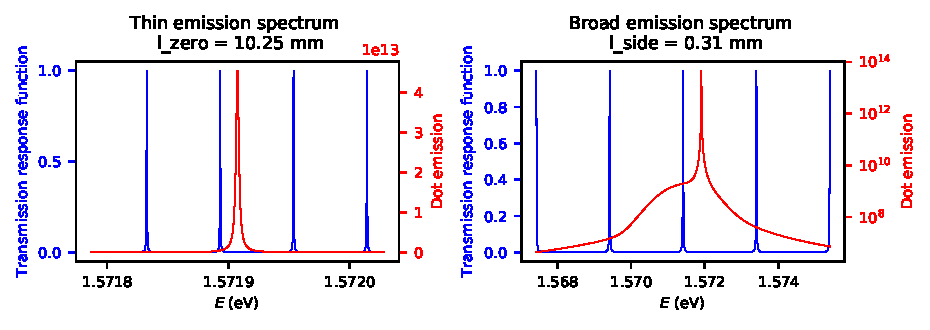
\includegraphics[width=\linewidth]{figures/plots/fabry-perot/simulation-comparison-dot-fabry-perot-modes}
	\caption{}
	\label{fig:simulation-comparison-dot-fabry-perot-modes}
\end{figure}


\Blindtext

\section{Setup}

\section{Measurements and Results}